\documentclass[12pt]{article}
\title{Understanding the Challenges of Evolving Multi-Agent Cooperation Using RWG Benchmarking}
\author{Mostafa Rizk}

\usepackage{graphicx}
\usepackage{subfig}
\usepackage[margin=1.5in]{geometry}
\usepackage{fancyhdr}
\usepackage{url}
\usepackage{tabu}
\usepackage[toc,page]{appendix}

\fancyhead{}
\fancyfoot{}
\fancyfoot[R]{\thepage}

\pagestyle{fancy}
\begin{document}
\maketitle
\tableofcontents

\section{Executive Summary}

We conducted an analysis of the SlopeForaging problem, described in Section \ref{experimental_setup} of the appendix, using Oller et al's rwg benchmarking approach \cite{oller:AAMAS:2020} to understand the types of challenges it poses and why it is difficult to evolve cooperative behaviour. 
We focused primarily on the role of the neural network architecture.
Our main insights were as follows:\\

Primary:
\begin{itemize}
\item The SlopeForaging task has similar attributes to MountainCar, meaning a highly exploratory algorithm may be more successful.

\item SlopeForaging is more difficult than MountainCar due to observation size, action space, partial observability and the cooperative nature of the task. 

\item An RNN architecture appears to be required for good performance but bias neurons don't make a difference.

\item Networks with non-linear activation are not as successful as those with linear activation but may get better with additional layers. 
This is most pronounced for tanh activation.

\item Deeper networks may be more adept at solving the task but it is difficult to tell because the solution space is much larger.

\item In order for a homogeneous team to exhibit specialisation, it might need to be able to switch between policies and remember how long it has been doing each one.
A network with long term memory may be necessary.

\end{itemize}

Secondary:
\begin{itemize}

\item The implementation contains some minor logical errors with regards to reward allocation and movement costs that should be modified for future experiments.
\end{itemize}

\section{Analysis}
		
We have faced difficulty evolving cooperation in the SlopeForaging multi-agent setting (described in Section \ref{experimental_setup}). 
We conducted an analysis using Oller et al's rwg benchmarking approach \cite{oller:AAMAS:2020} to understand the nature of the difficulties posed by this environment. 
We hope this will provide insight into what changes need to be made to our approach in order to produce the desired behaviour. 
All experiments used a heterogeneous team, rewarded at the team level. 
We initially used homogeneous teams but found that they add a layer of difficulty to the problem.
Both homogeneous teams and individual rewards will be considered at a later stage.\\

In each experiment, we sampled 50,000 genomes from a normal distribution with a mean of 0 and unit variance.
We chose to use 50,000 samples rather than 10,000 as in Oller et al because this is a more difficult task to solve, which we discuss further in Section \ref{task_difficulty}.
Each genome was evaluated for 5 episodes. 
In any instance where hidden layers were used, we used 4 hidden units. 
We plot a) all the trials in sorted order by score, b) the variance of all trials and c) the distribution on a log scale.\\

We started our experiments with the simplest possible architecture, a FFNN with no bias, no hidden layers and linear activation (i.e. the identity function). 
We added up to two hidden layers, then repeated with bias, making for a total of 6 experiments. 
We then repeated the 6 experiments with a RNN. \\

For the FFNN, the scores are overwhelmingly poor in comparison to RNNs. 
We also learned, after the experiments, that according to Theorem 1.5.1 in \cite{aggarwal:Springer:2018}, that hidden layers do not add computational power if the activation function is linear. 
We therefore chose to exclude those plots and repeated these experiments in Section \ref{non-linear} with various non-linear activations.
For brevity we put the FFNN plots and analysis in the appendix in Section \ref{FFNN}. \\

The organisation of this report is as follows: 
Section \ref{task_difficulty} discusses the fundamental difficulties of the task using Oller et al's analysis of MountainCar \cite{MountainCar} as a reference. 
Section \ref{RNN Architecture} talks about why a recurrent network appears to be necessary. 
Section \ref{non-linear} explores the impact of non-linear activation functions on performance. 
Section \ref{tanh_multilayer} does a preliminary analysis of the benefit of additional layers. 
Section \ref{lazy_generalist} uses additional experiments to examine what may be the minimum requirements of a neural network used in this task. 
Finally Section \ref{conclusion} summarises our findings and proposes our next steps. \\ 

\subsection{Task Difficulty} \label{task_difficulty}

On a fundamental level, we learn from these experiments that the environment, independent of architecture, is challenging in a way that is similar to the MountainCar environment  \cite{MountainCar} investigated by Oller et al \cite{oller:AAMAS:2020}. 
The plots are very similar with most solutions being equally poor and very few demonstrating a successful behaviour. 
We see this in Figure \ref{fig:rnn_linear} that the mean curve is very flat with a spike at the end, indicating there are a small number of high performing solutions while the rest score below 0.
This can also be seen in the distribution histogram, to the right, where the majority of solutions fall in the leftmost bucket for scores below 0. 
The variance plot, in the center, shows that variance is higher for higher means suggesting that genomes that score well do not do so consistently across all episodes.\\

The reason most solutions score very poorly is likely because both the SlopeForaging and MountainCar environments have a sparse reward. 
In the case of MountainCar, an agent must reach the top of the mountain to receive a score better than -200 and there are no rewards for partially successful intermediate behaviours. 
An agent that never moves is equivalent to one that stops just short of the goal. 
In SlopeForaging, an agent that travels up the slope, picks up a resource, carries it to the bottom of the slope and drops it just short of the nest is equivalent to an agent that oscillates back and forth between two tiles. 
A non-negative score can only be achieved if a resource is fully retrieved and there are no rewards for partially successful intermediate behaviours, so the task can not be learned incrementally.\\

In fact, the SlopeForaging task is actually more difficult for the following reasons:

\begin{itemize}
\item \textit{The observation and action spaces are larger}- An observation consists of 41 binary inputs and there are 6 discrete actions. 
Even the simplest FFNN would have 41x6=246 weights compared to (2x4) + (4x4) + (4x3) = 36 for the most complex controller used by Oller et al to solve MountainCar. 

\item \textit{The environment is partially observable}- Partial observability suggests that a more complex architecture, such as an RNN, may be required as stated by Oller et al \cite{oller:AAMAS:2020}.

\item \textit{The best solution isn't found even after 50,000 samples}- In MountainCar \cite{MountainCar}, the theoretical best score is close to 0 and the solutions generated by Oller et al approach this value, whereas in SlopeForaging, a team of specialists hardcoded with a cooperative strategy scores 157,711 but the best mean score of the solutions found by rwg is 6065 (39,879 for a homogeneous setup). 
This is very far from the best known solution. 
It is even far from the best known generalist strategy, which scores 118,353. 
And all this is with 5 times more sampled solutions than Oller et al. 
All this is to say, the task is difficult to solve and, according to Oller et al's recommendations, may require an algorithm with a strong exploratory component.

\end{itemize}

\textbf{Main takeaway: The SlopeForaging task has similar attributes to MountainCar but is more difficult due to observation size, action space, partial observability and the cooperative nature of the task.}
		
\subsection{Recurrent Networks and Memory} \label{RNN Architecture}

As stated at the beginning of the section, RNNs were found to outperform FFNNs. 
This makes sense because the environment is partially observable; an agent can only see 1 tile in any direction. 
A recurrent architecture means an agent can act on its observation while also knowing the action it took in the previous time step.
This gives it a form of memory, meaning it is effectively able to act on sequences of observations rather than individual observations, giving it an advantage over an agent with no memory. 
Presumably, if the agent's sensing radius was expanded to include the entire arena then the FFNN would perform similarly to the RNN. \\ 

\textbf{Main takeaway: Memory appears to be required for good performance.}


\begin{figure}[!tbp]
  \centering
  % RNN no-bias 0HL
  \subfloat{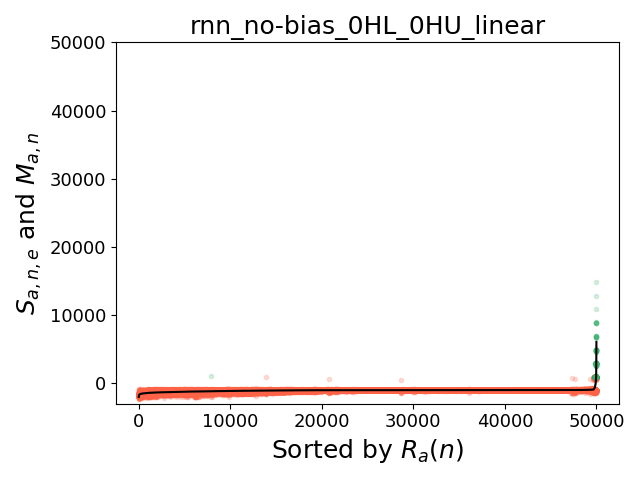
\includegraphics[width=0.3\textwidth]{rnn_no-bias_0HL/rnn_no-bias_0HL_score_trials_ordered_.png}}
  \hfill
  \subfloat{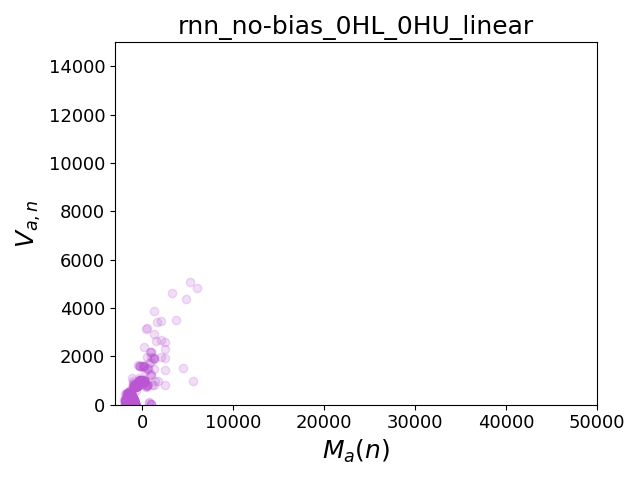
\includegraphics[width=0.3\textwidth]{rnn_no-bias_0HL/rnn_no-bias_0HL_variance_meanscore_.png}}
  \hfill
  \subfloat{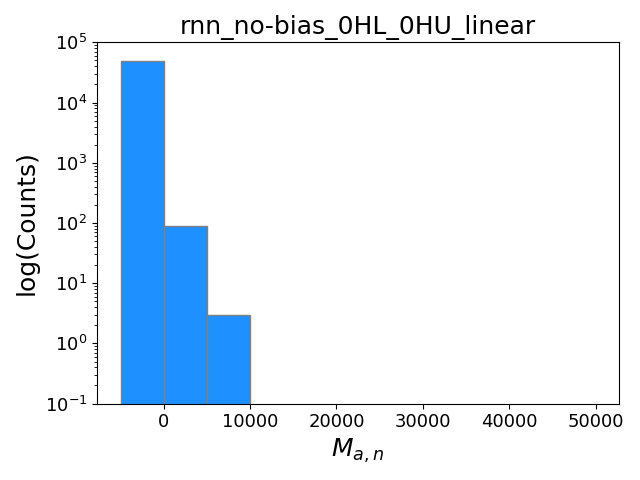
\includegraphics[width=0.3\textwidth]{rnn_no-bias_0HL/rnn_no-bias_0HL_all_scores_log_dist_.png}}
  
% RNN bias 0HL
%  \subfloat{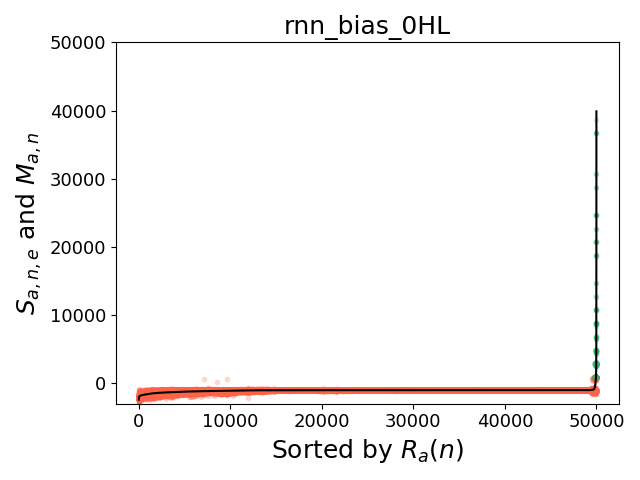
\includegraphics[width=0.3\textwidth]{rnn_bias_0HL/rnn_bias_0HL_score_trials_ordered_.png}}
%  \hfill
%  \subfloat{\includegraphics[width=0.3\textwidth]{rnn_bias_0HL/%rnn_bias_0HL_variance_meanscore_.png}}
%  \hfill
%  \subfloat{\includegraphics[width=0.3\textwidth]{rnn_bias_0HL/%rnn_bias_0HL_all_scores_log_dist_.png}}
  
 \caption{RNN with linear activation}
 \label{fig:rnn_linear}	
\end{figure}	

%%%
	
					
\subsection{Non-linear Activation}\label{non-linear}

Following the results from Section \ref{RNN Architecture} we conducted the same experiments with non-linear activations, specifically tanh, ReLU and sigmoid functions. 
We primarily looked at RNNs because previous experiments indicated that an RNN architecture may be necessary for successful behaviour, but we included a FFNN with tanh activation for due diligence in Section \ref{ffnn_non-linear} of the appendix. 
For the three activations, as before, we did six experiments, three with bias and three without, and of those three we tested 0, 1 and 2 hidden layers, with 4 hidden units.
We found no difference between networks with and without bias so we moved the bias plots to Section \ref{rnn_non-linear_bias} of the appendix.\\

For all three activations, the highest scores are lower than they are for linear activation. 
This is surprising as one would expect non-linear activation to provide more representational power to the neural network. 
Interestingly, though, for tanh and ReLU (Figures \ref{fig:rnn_tanh} and \ref{fig:rnn_relu} respectively) the instances of high scores (and the top score) show some increase while sigmoid activation (Figure \ref{fig:rnn_sigmoid}) does not. 
This suggests that while a network with linear activation is more successful with no hidden layers than its counterparts, the networks with tanh and ReLU activation gain representational power and their performance improves with additional layers. 
In the histograms in Figure \ref{fig:rnn_relu}, the difference between layers is not as visible as it is for Figure \ref{fig:rnn_tanh} but can be seen in the top scores in Table \ref{tab:architecture_comparison}. 
This suggests that the added gain of each new layer is greater for networks using tanh than networks using ReLU.\\

In both cases, though, it is unclear if there would be an upward trend with more hidden layers, or if varying the number of hidden units would accelerate the improvement or if there is another activation function for which the improvement is more pronounced. 
Additional rwg runs with these deeper architectures can help answer these questions but may also reach a bottleneck as additional layers means more weights, increasing the size of the solution space. 
Some form of topological search \cite{stanley:MIT:2002} is another way of discovering which architecture is most capable of representing problem solutions.\\ 

Sigmoid activation was the exception to the trend, with the distribution of RNN solutions in Figure \ref{fig:rnn_sigmoid} being similar to those of FFNNs with linear activation in Figure \ref{fig:ffnn_linear}. 
Networks with sigmoid activation appear to not have the representational power required to solve the problem, but it is unclear why. 
The same holds true for FFNNs with tanh activation (Figure \ref{fig:ffnn_tanh}). 
For all networks, though, bias neurons did not make a notable difference.\\

\begin{figure}[!tbp]
  \centering
  % RNN no-bias 0HL
  \subfloat{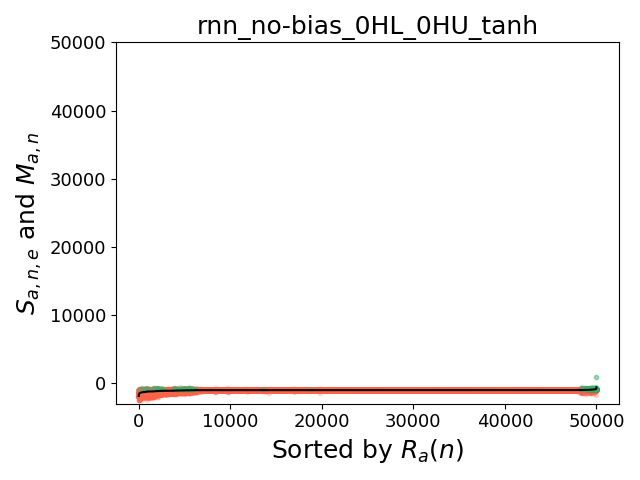
\includegraphics[width=0.3\textwidth]{rnn_no-bias_0HL_tanh/rnn_no-bias_0HL_tanh_score_trials_ordered_.png}}
  \hfill
  \subfloat{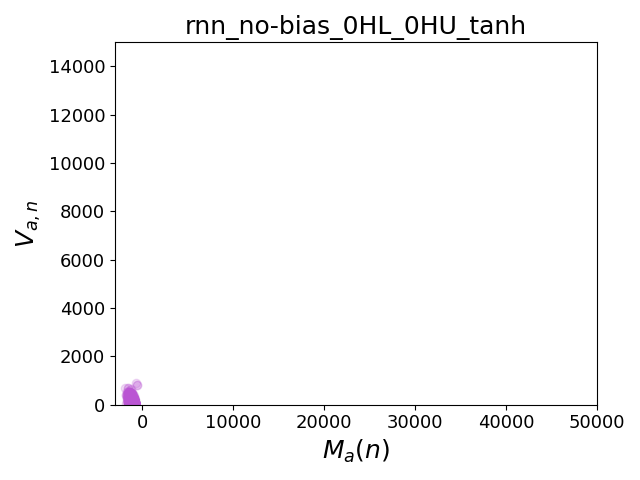
\includegraphics[width=0.3\textwidth]{rnn_no-bias_0HL_tanh/rnn_no-bias_0HL_tanh_variance_meanscore_.png}}
  \hfill
  \subfloat{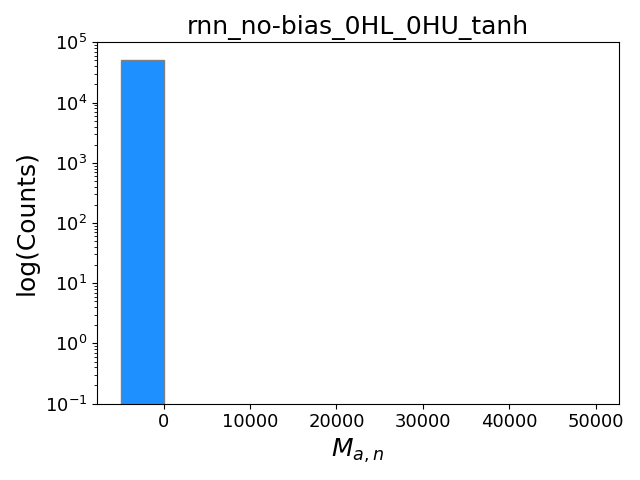
\includegraphics[width=0.3\textwidth]{rnn_no-bias_0HL_tanh/rnn_no-bias_0HL_tanh_all_scores_log_dist_.png}}
  
  % RNN no-bias 1HL
  \subfloat{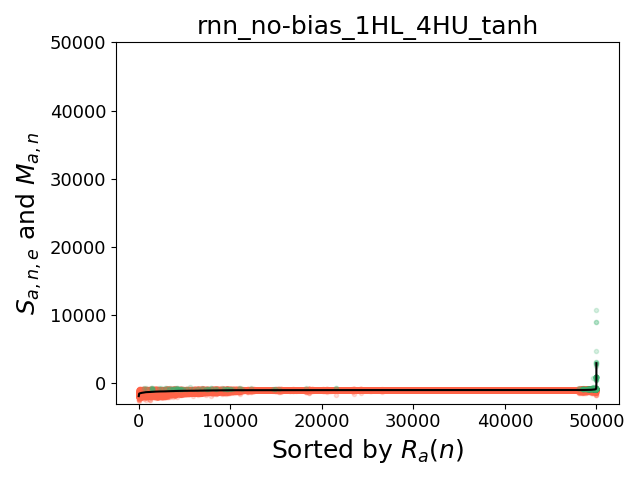
\includegraphics[width=0.3\textwidth]{rnn_no-bias_1HL_4HU_tanh/rnn_no-bias_1HL_4HU_tanh_score_trials_ordered_.png}}
  \hfill
  \subfloat{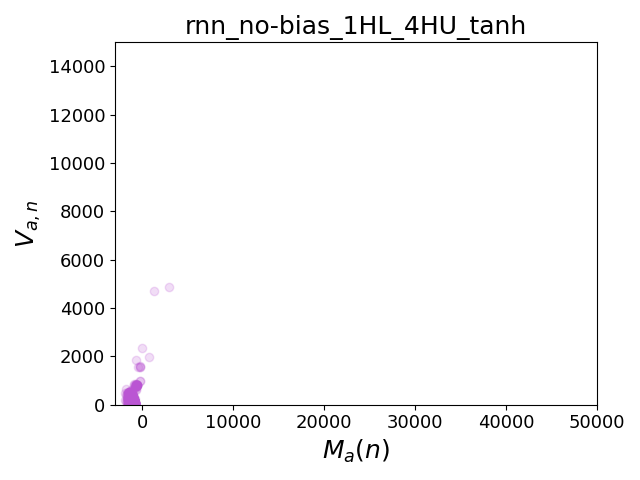
\includegraphics[width=0.3\textwidth]{rnn_no-bias_1HL_4HU_tanh/rnn_no-bias_1HL_4HU_tanh_variance_meanscore_.png}}
  \hfill
  \subfloat{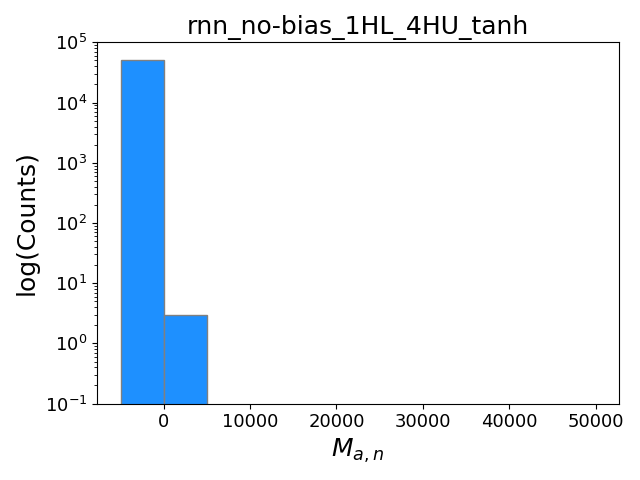
\includegraphics[width=0.3\textwidth]{rnn_no-bias_1HL_4HU_tanh/rnn_no-bias_1HL_4HU_tanh_all_scores_log_dist_.png}}

% RNN no-bias 2HL
  \subfloat{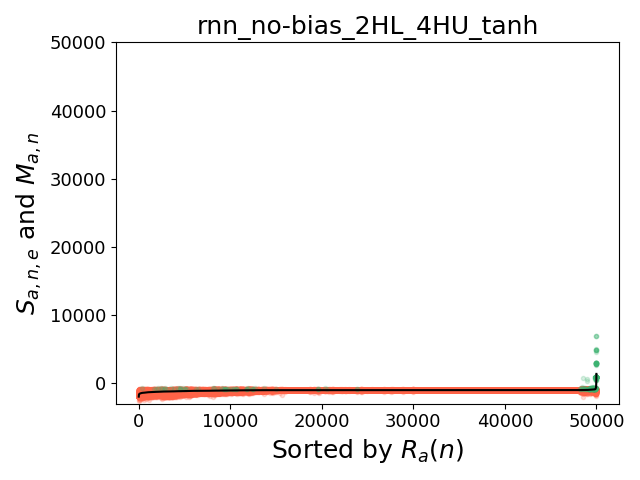
\includegraphics[width=0.3\textwidth]{rnn_no-bias_2HL_4HU_tanh/rnn_no-bias_2HL_4HU_tanh_score_trials_ordered_.png}}
  \hfill
  \subfloat{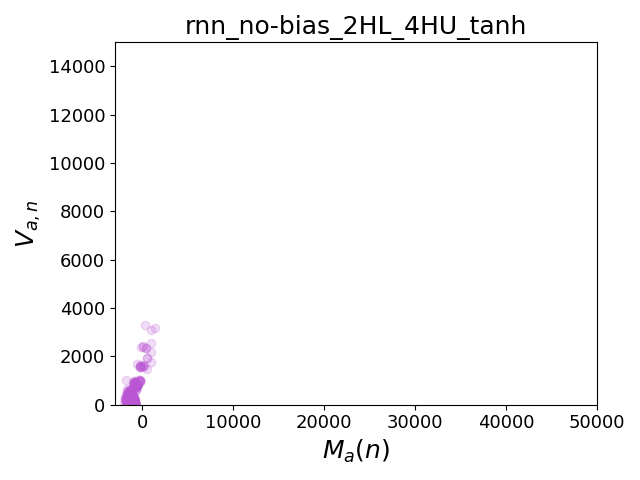
\includegraphics[width=0.3\textwidth]{rnn_no-bias_2HL_4HU_tanh/rnn_no-bias_2HL_4HU_tanh_variance_meanscore_.png}}
  \hfill
  \subfloat{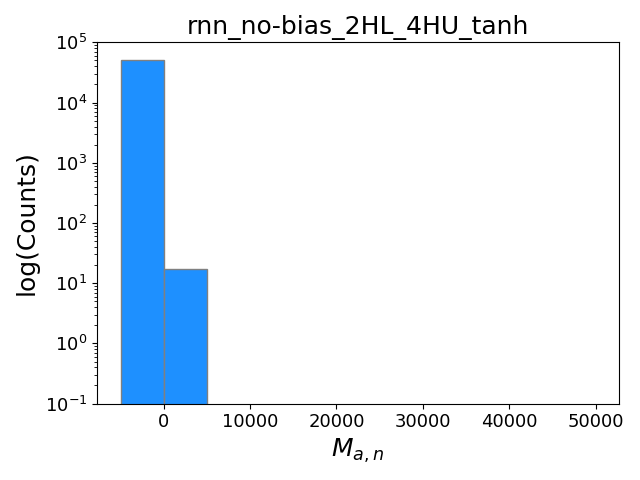
\includegraphics[width=0.3\textwidth]{rnn_no-bias_2HL_4HU_tanh/rnn_no-bias_2HL_4HU_tanh_all_scores_log_dist_.png}}
  
  \caption{RNN with tanh activation}
  \label{fig:rnn_tanh}	
\end{figure}	

\begin{figure}[!tbp]
  \centering
  % RNN no-bias 0HL
  \subfloat{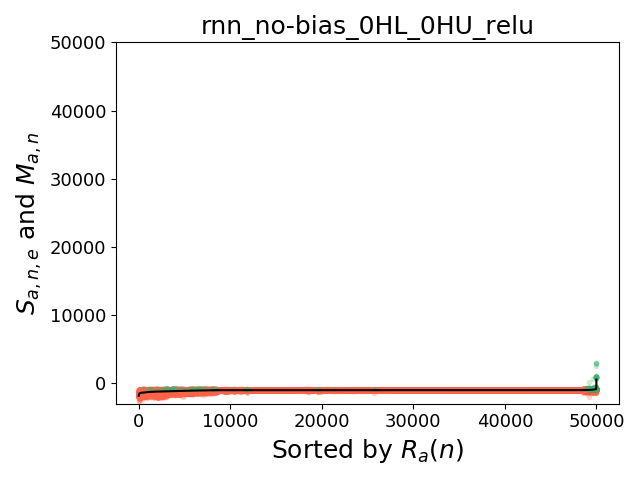
\includegraphics[width=0.3\textwidth]{rnn_no-bias_0HL_relu/rnn_no-bias_0HL_relu_score_trials_ordered_.png}}
  \hfill
  \subfloat{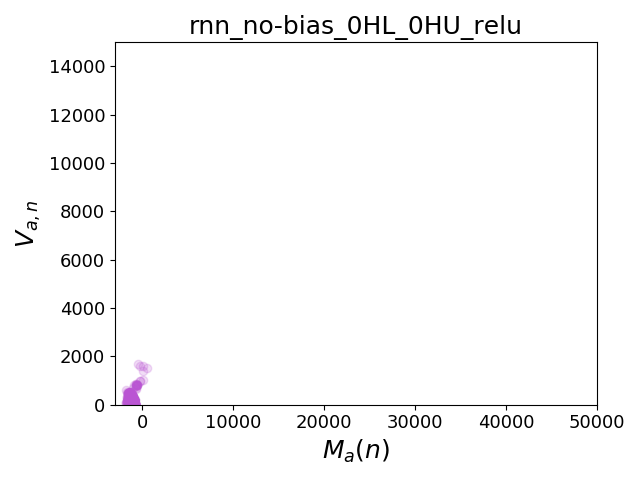
\includegraphics[width=0.3\textwidth]{rnn_no-bias_0HL_relu/rnn_no-bias_0HL_relu_variance_meanscore_.png}}
  \hfill
  \subfloat{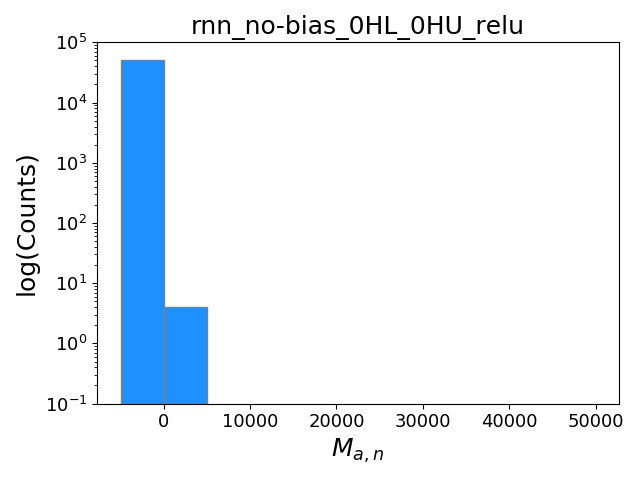
\includegraphics[width=0.3\textwidth]{rnn_no-bias_0HL_relu/rnn_no-bias_0HL_relu_all_scores_log_dist_.png}}
  
  % RNN no-bias 1HL
  \subfloat{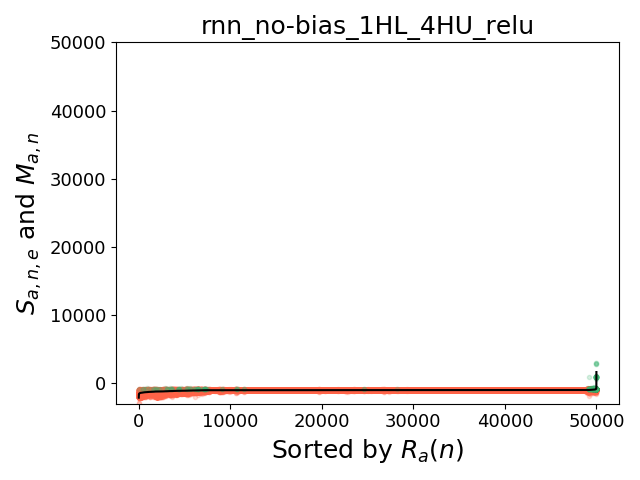
\includegraphics[width=0.3\textwidth]{rnn_no-bias_1HL_4HU_relu/rnn_no-bias_1HL_4HU_relu_score_trials_ordered_.png}}
  \hfill
  \subfloat{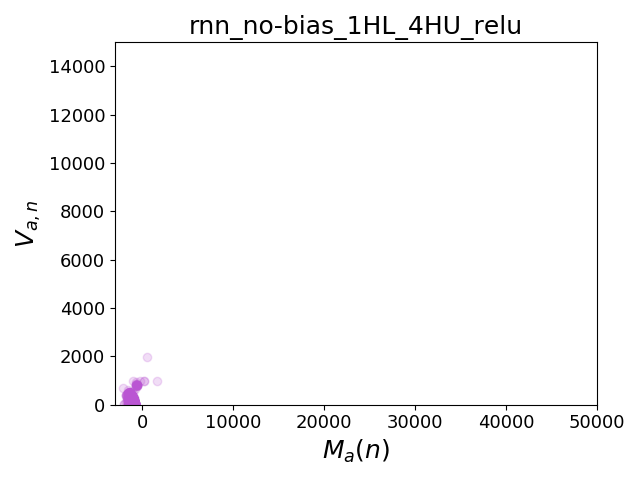
\includegraphics[width=0.3\textwidth]{rnn_no-bias_1HL_4HU_relu/rnn_no-bias_1HL_4HU_relu_variance_meanscore_.png}}
  \hfill
  \subfloat{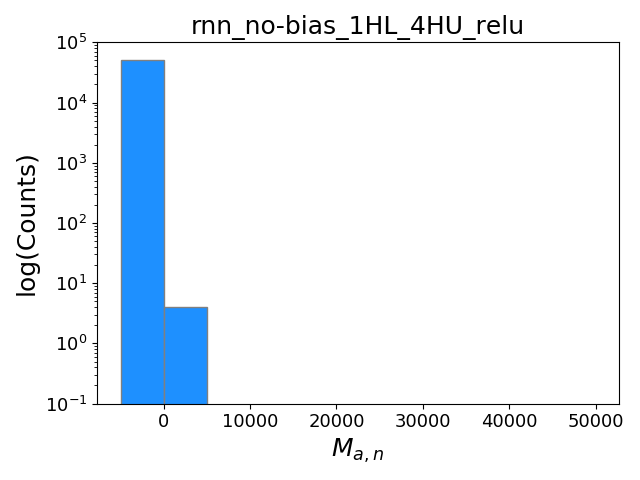
\includegraphics[width=0.3\textwidth]{rnn_no-bias_1HL_4HU_relu/rnn_no-bias_1HL_4HU_relu_all_scores_log_dist_.png}}

% RNN no-bias 2HL
  \subfloat{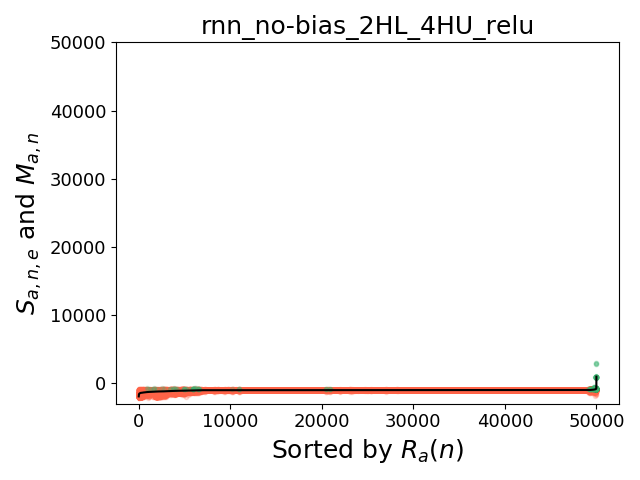
\includegraphics[width=0.3\textwidth]{rnn_no-bias_2HL_4HU_relu/rnn_no-bias_2HL_4HU_relu_score_trials_ordered_.png}}
  \hfill
  \subfloat{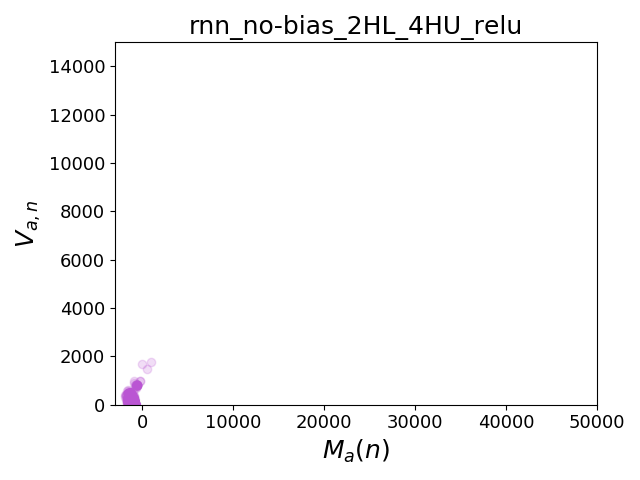
\includegraphics[width=0.3\textwidth]{rnn_no-bias_2HL_4HU_relu/rnn_no-bias_2HL_4HU_relu_variance_meanscore_.png}}
  \hfill
  \subfloat{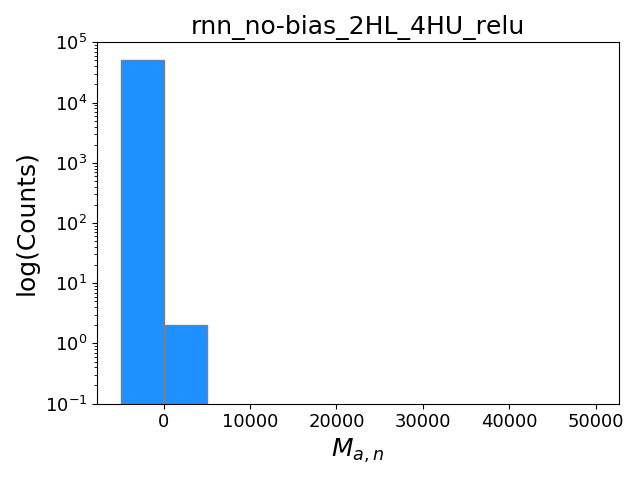
\includegraphics[width=0.3\textwidth]{rnn_no-bias_2HL_4HU_relu/rnn_no-bias_2HL_4HU_relu_all_scores_log_dist_.png}}
  
  \caption{RNN with ReLU activation}
  \label{fig:rnn_relu}	
\end{figure}	

\begin{figure}[!tbp]
  \centering
  % RNN no-bias 0HL
  \subfloat{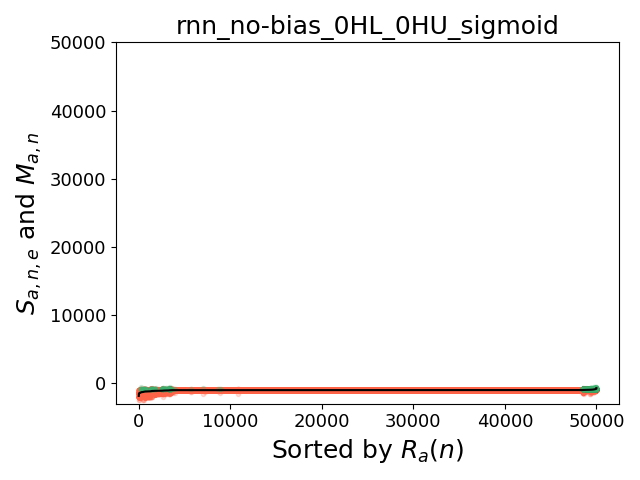
\includegraphics[width=0.3\textwidth]{rnn_no-bias_0HL_sigmoid/rnn_no-bias_0HL_sigmoid_score_trials_ordered_.png}}
  \hfill
  \subfloat{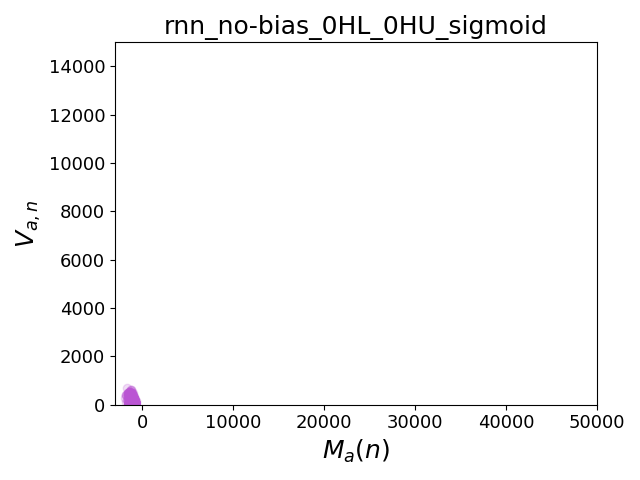
\includegraphics[width=0.3\textwidth]{rnn_no-bias_0HL_sigmoid/rnn_no-bias_0HL_sigmoid_variance_meanscore_.png}}
  \hfill
  \subfloat{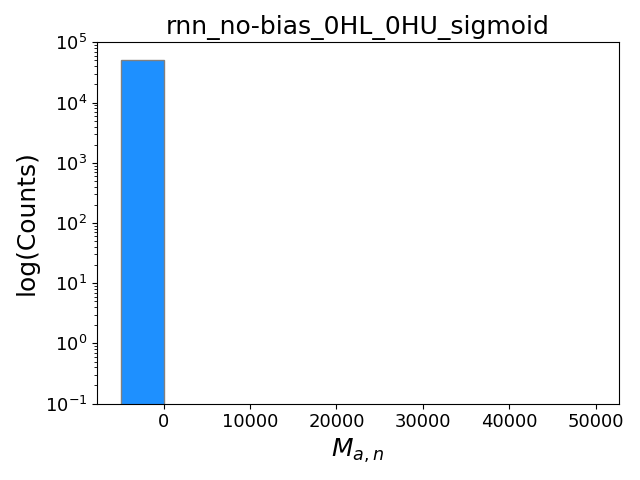
\includegraphics[width=0.3\textwidth]{rnn_no-bias_0HL_sigmoid/rnn_no-bias_0HL_sigmoid_all_scores_log_dist_.png}}
  
  % RNN no-bias 1HL
  \subfloat{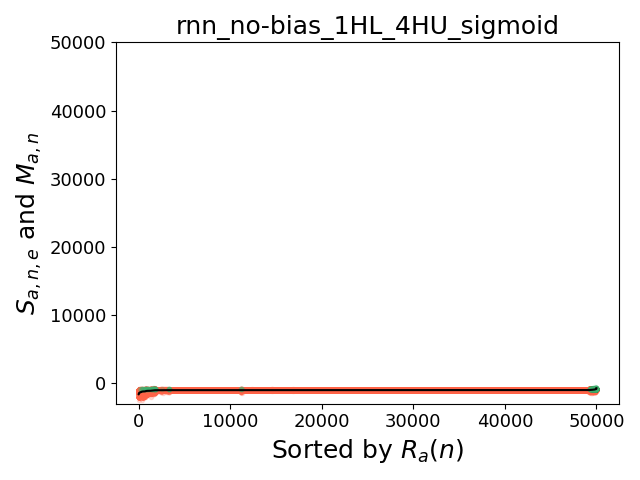
\includegraphics[width=0.3\textwidth]{rnn_no-bias_1HL_4HU_sigmoid/rnn_no-bias_1HL_4HU_sigmoid_score_trials_ordered_.png}}
  \hfill
  \subfloat{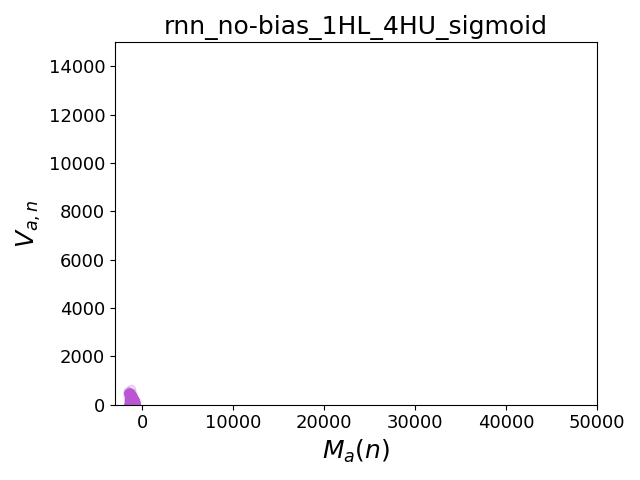
\includegraphics[width=0.3\textwidth]{rnn_no-bias_1HL_4HU_sigmoid/rnn_no-bias_1HL_4HU_sigmoid_variance_meanscore_.png}}
  \hfill
  \subfloat{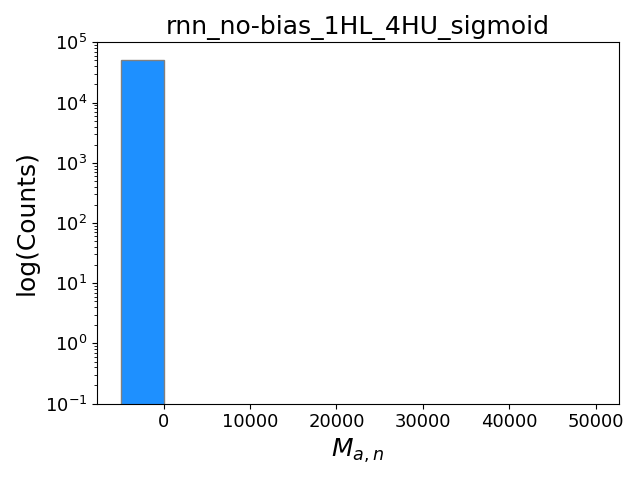
\includegraphics[width=0.3\textwidth]{rnn_no-bias_1HL_4HU_sigmoid/rnn_no-bias_1HL_4HU_sigmoid_all_scores_log_dist_.png}}

% RNN no-bias 2HL
  \subfloat{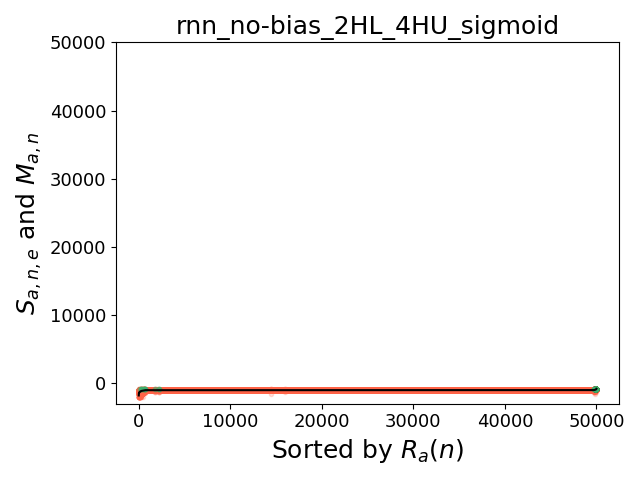
\includegraphics[width=0.3\textwidth]{rnn_no-bias_2HL_4HU_sigmoid/rnn_no-bias_2HL_4HU_sigmoid_score_trials_ordered_.png}}
  \hfill
  \subfloat{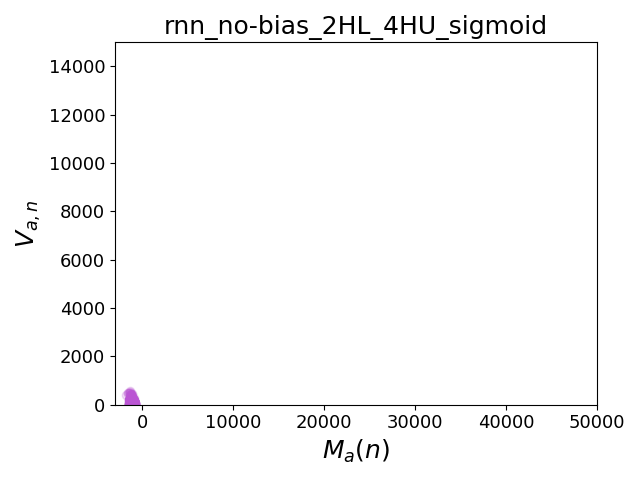
\includegraphics[width=0.3\textwidth]{rnn_no-bias_2HL_4HU_sigmoid/rnn_no-bias_2HL_4HU_sigmoid_variance_meanscore_.png}}
  \hfill
  \subfloat{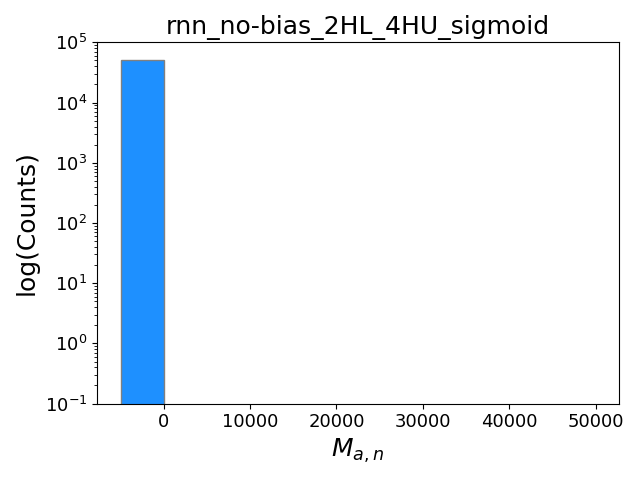
\includegraphics[width=0.3\textwidth]{rnn_no-bias_2HL_4HU_sigmoid/rnn_no-bias_2HL_4HU_sigmoid_all_scores_log_dist_.png}}
  
  \caption{RNN with sigmoid activation}
  \label{fig:rnn_sigmoid}	
\end{figure}	

\begin{table}
\begin{center}
\begin{tabu}{ |c|c|c|c|c|c| } 
 \hline
 Network Type & Layers & Bias & Activation & Top Hom Score & Top Het Score\\
 \tabucline[1.5pt]{-}
 FFNN & 0 & N & Linear & -620 & -721 \\
 \hline
 FFNN & 0 & Y & Linear & -620 & \\
 \tabucline[1.5pt]{-}
 
 RNN & 0 & N & Linear & 39879 & 6065 \\
 \hline
 RNN & 0 & Y & Linear & 39879 & \\
 \tabucline[1.5pt]{-}
 
 RNN & 0 & N & tanh & 297 & -608 \\
 \hline
 RNN & 1 & N & tanh & 3361 & 2942 \\
 \hline
 RNN & 2 & N & tanh & 8376 & 1372 \\
 \hline
 RNN & 0 & Y & tanh & 297 & -608 \\
 \hline
 RNN & 1 & Y & tanh & 3361 & 2942 \\
 \hline
 RNN & 2 & Y & tanh & 8376 & 1372 \\
 \tabucline[1.5pt]{-}
 
 RNN & 0 & N & ReLU & 1375 & 542 \\
 \hline
 RNN & 1 & N & ReLU & 2402 & 1645 \\
 \hline
 RNN & 2 & N & ReLU & 5224 & 971 \\
 \hline
 RNN & 0 & Y & ReLU & 1375 & 542 \\
 \hline
 RNN & 1 & Y & ReLU & 2402 & 1645 \\
 \hline
 RNN & 2 & Y & ReLU & 5224 & 971 \\
 \tabucline[1.5pt]{-}
 
 RNN & 0 & N & sigmoid & -610 & -720 \\
 \hline
 RNN & 1 & N & sigmoid & -603 & -736 \\
 \hline
 RNN & 2 & N & sigmoid & -620 & -810 \\
 \hline
 RNN & 0 & Y & sigmoid & -610 & -720 \\
 \hline
 RNN & 1 & Y & sigmoid & -603 & -736 \\
 \hline
 RNN & 2 & Y & sigmoid & -620 & -810 \\
 \tabucline[1.5pt]{-}

 FFNN & 0 & N & tanh & -620 & -721 \\
 \hline
 FFNN & 1 & N & tanh & -609 & -774 \\
 \hline
 FFNN & 2 & N & tanh & -620 & -775 \\
 \hline
 FFNN & 0 & Y & tanh & -620 & -721 \\
 \hline
 FFNN & 1 & Y & tanh & -609 & -774 \\
 \hline
 FFNN & 2 & Y & tanh & -620 & -775 \\
 \tabucline[1.5pt]{-}
 \hline
\end{tabu}
\end{center}	
\caption{\label{tab:architecture_comparison} Top scores with different architectures}
\end{table}

\textbf{Main takeaway: Networks with non-linear activation are not as successful as those with linear activation but may get better with additional layers. 
This is most pronounced for tanh activation. }

\subsection{Adding Layers} \label{tanh_multilayer}

As noted in the previous section, networks with tanh activation seem to yield more high performing solutions as the number of hidden layers increases. 
To investigate this further, we ran additional experiments, using tanh activation, no bias and 3, 4, 5, 6 and 7 hidden layers.
We found that while the quality of solutions appeared to increase between 0, 1 and 2 hidden layers, this trend does not continue for additional layers.
We can see in the histograms in Figure \ref{fig:tanh_multilayer} that all solutions fall into the first 2 buckets.
Higher top scores are thus not found, which we also see in Table \ref{tab:architecture_comparison_tanh} where the highest score fluctuates, suggesting that the distribution does not shift significantly.\\

The height of the second bucket in the histogram plots approaches $10^2$ for the 7-layer network, whereas it is close to $10^1$ for the 2-layer network and even smaller for the smaller networks.
Further increasing the number of layers does in fact allow us to find more solutions of higher quality, but the number is only on the order of tens.
However, it is important to view this in the context of the larger solution space (due to the larger genome size).
A network with 2 hidden layers has 260 weights, whereas one with 7 hidden layers has 420.
RWG was able to find tens more solutions that fit in the second bucket, but there are also many more possible solutions to sample. 
It is possible that in the solution space for a 7-hidden layer network there is a larger number of successful architectures but they are harder to find by sampling. 
The RWG approach may be limited in its ability to analyse task difficulty for applications with larger neural networks.
Further analysis may require alternative techniques.\\

\textbf{Main takeaway: Deeper networks may be more adept at solving the task but it is difficult to tell because the solution space is much larger. }

\begin{figure}[!tbp]
  \centering
  % RNN no-bias 3HL 
  \subfloat{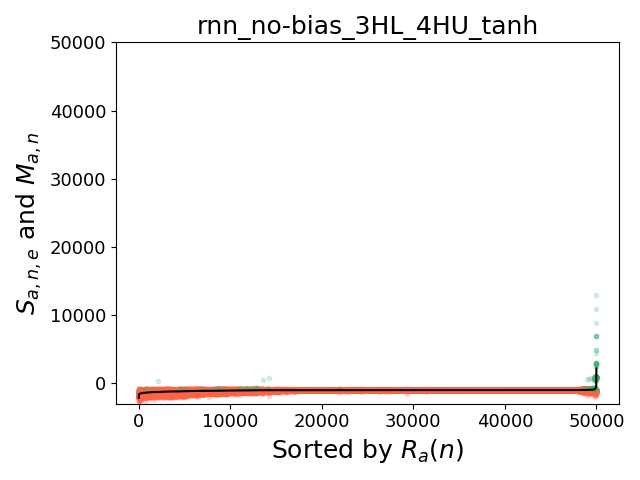
\includegraphics[width=0.3\textwidth]{rnn_no-bias_3HL_4HU_tanh/rnn_no-bias_3HL_4HU_tanh_score_trials_ordered_.png}}
  \hfill
  \subfloat{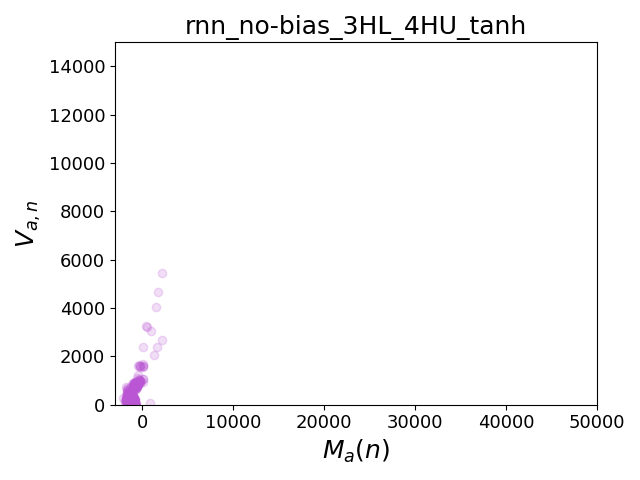
\includegraphics[width=0.3\textwidth]{rnn_no-bias_3HL_4HU_tanh/rnn_no-bias_3HL_4HU_tanh_variance_meanscore_.png}}
  \hfill
  \subfloat{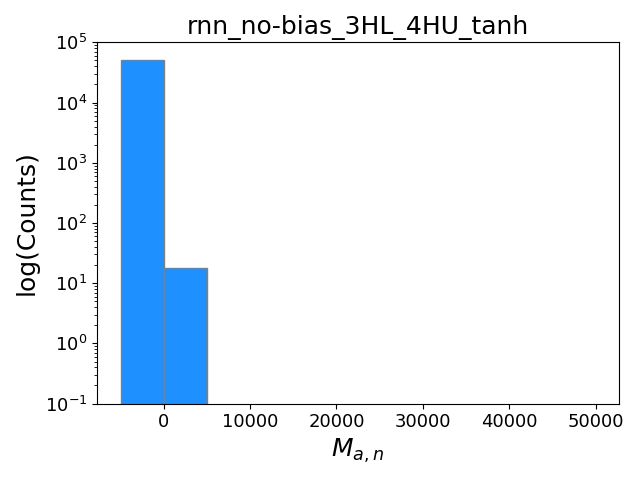
\includegraphics[width=0.3\textwidth]{rnn_no-bias_3HL_4HU_tanh/rnn_no-bias_3HL_4HU_tanh_all_scores_log_dist_.png}}
  
  % RNN no-bias 4HL 
  \subfloat{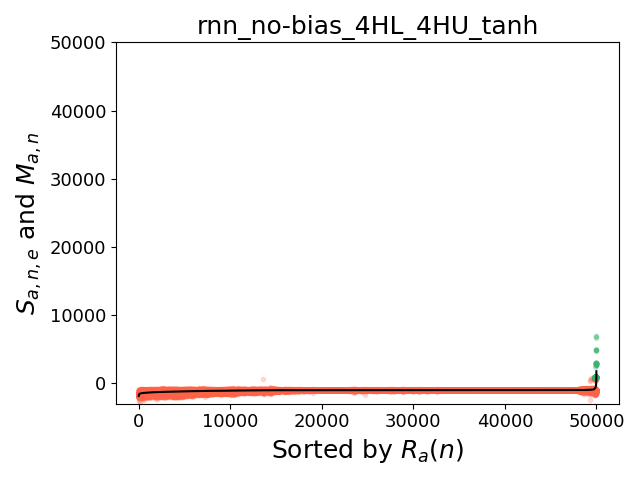
\includegraphics[width=0.3\textwidth]{rnn_no-bias_4HL_4HU_tanh/rnn_no-bias_4HL_4HU_tanh_score_trials_ordered_.png}}
  \hfill
  \subfloat{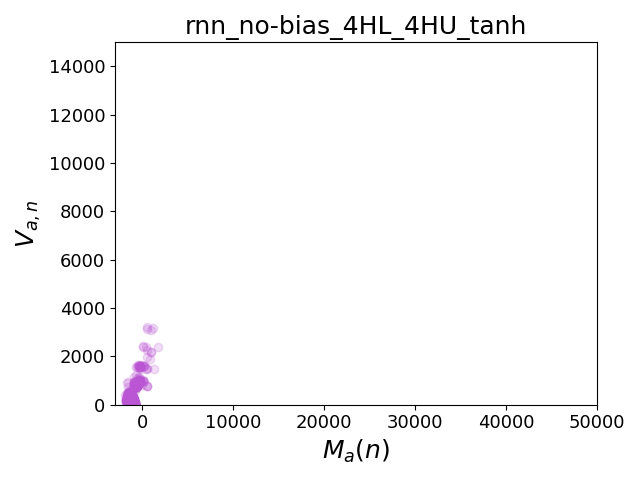
\includegraphics[width=0.3\textwidth]{rnn_no-bias_4HL_4HU_tanh/rnn_no-bias_4HL_4HU_tanh_variance_meanscore_.png}}
  \hfill
  \subfloat{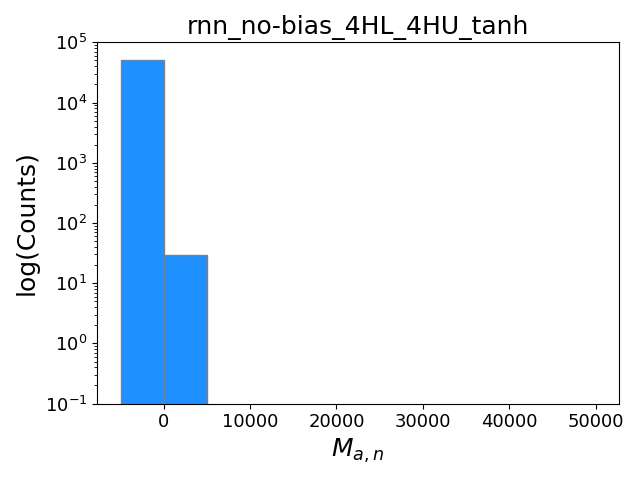
\includegraphics[width=0.3\textwidth]{rnn_no-bias_4HL_4HU_tanh/rnn_no-bias_4HL_4HU_tanh_all_scores_log_dist_.png}}

% RNN no-bias 5HL 
  \subfloat{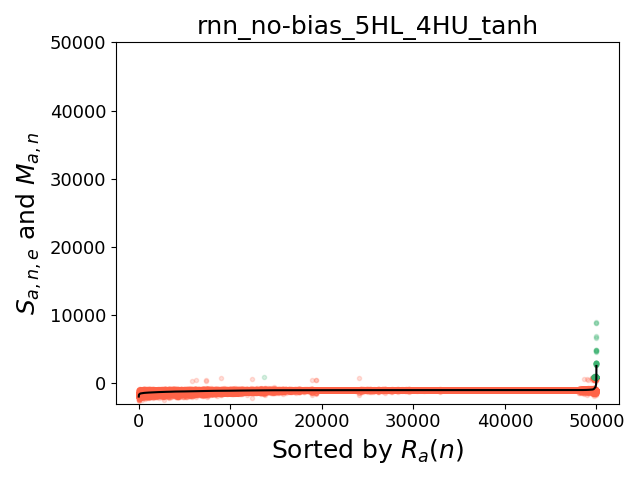
\includegraphics[width=0.3\textwidth]{rnn_no-bias_5HL_4HU_tanh/rnn_no-bias_5HL_4HU_tanh_score_trials_ordered_.png}}
  \hfill
  \subfloat{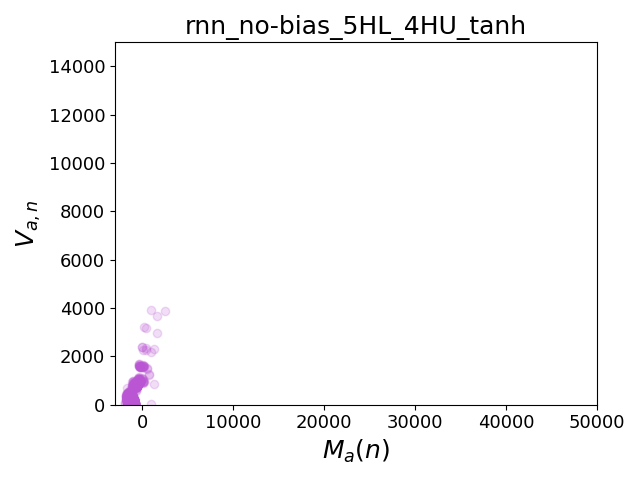
\includegraphics[width=0.3\textwidth]{rnn_no-bias_5HL_4HU_tanh/rnn_no-bias_5HL_4HU_tanh_variance_meanscore_.png}}
  \hfill
  \subfloat{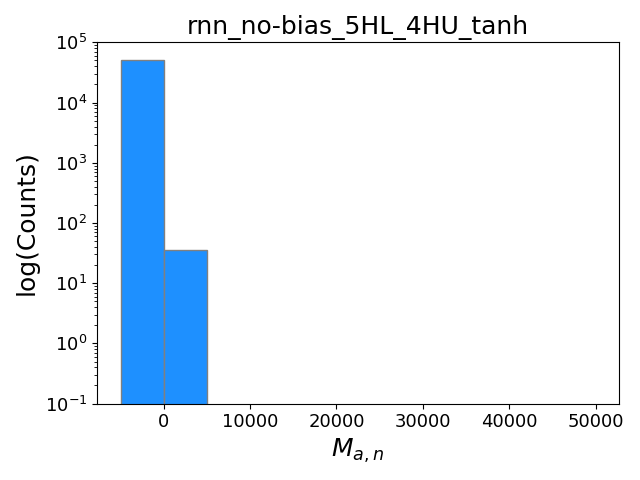
\includegraphics[width=0.3\textwidth]{rnn_no-bias_5HL_4HU_tanh/rnn_no-bias_5HL_4HU_tanh_all_scores_log_dist_.png}}

  % RNN no-bias 6HL 
  \subfloat{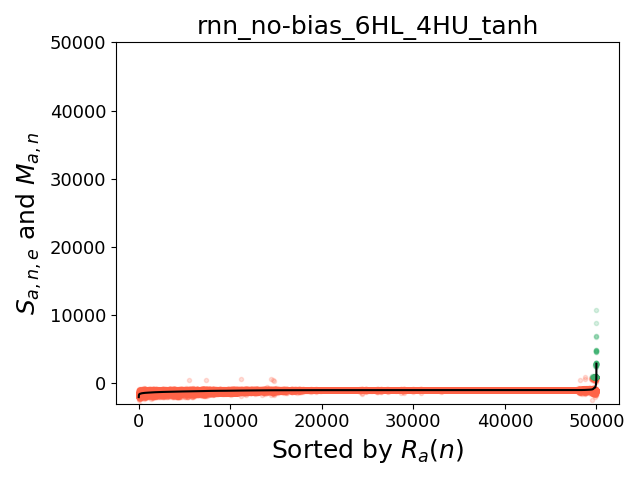
\includegraphics[width=0.3\textwidth]{rnn_no-bias_6HL_4HU_tanh/rnn_no-bias_6HL_4HU_tanh_score_trials_ordered_.png}}
  \hfill
  \subfloat{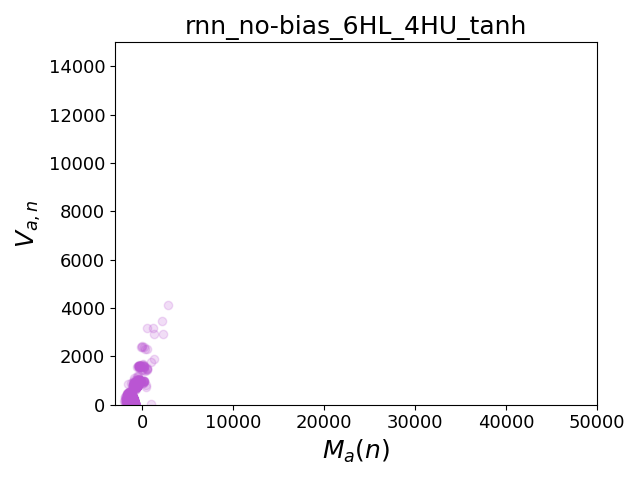
\includegraphics[width=0.3\textwidth]{rnn_no-bias_6HL_4HU_tanh/rnn_no-bias_6HL_4HU_tanh_variance_meanscore_.png}}
  \hfill
  \subfloat{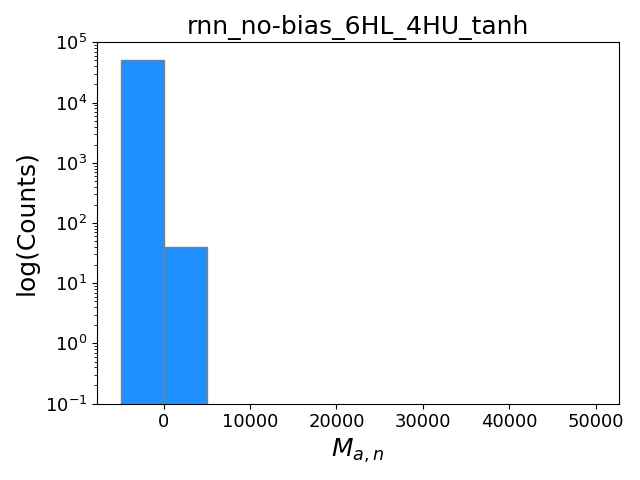
\includegraphics[width=0.3\textwidth]{rnn_no-bias_6HL_4HU_tanh/rnn_no-bias_6HL_4HU_tanh_all_scores_log_dist_.png}}

  % RNN no-bias 7HL 
  \subfloat{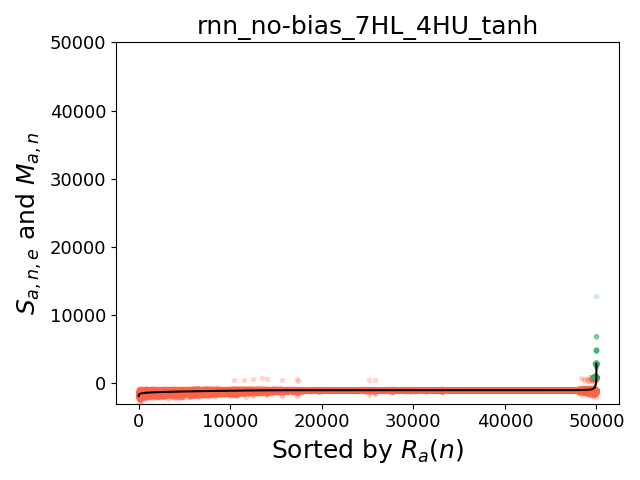
\includegraphics[width=0.3\textwidth]{rnn_no-bias_7HL_4HU_tanh/rnn_no-bias_7HL_4HU_tanh_score_trials_ordered_.png}}
  \hfill
  \subfloat{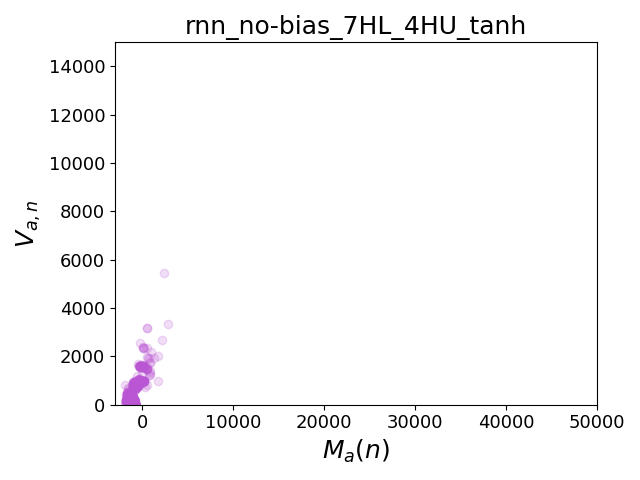
\includegraphics[width=0.3\textwidth]{rnn_no-bias_7HL_4HU_tanh/rnn_no-bias_7HL_4HU_tanh_variance_meanscore_.png}}
  \hfill
  \subfloat{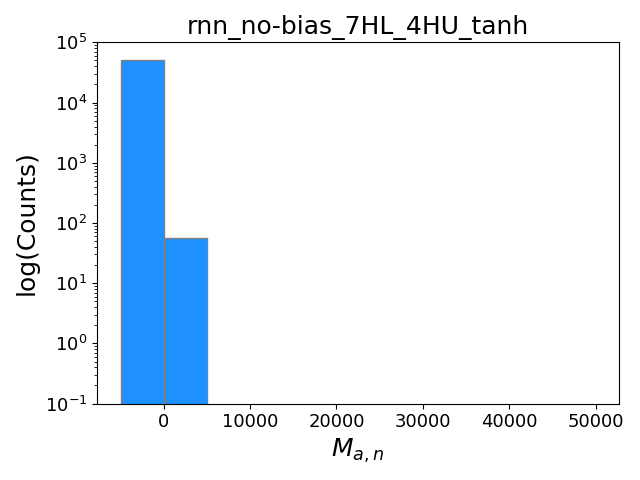
\includegraphics[width=0.3\textwidth]{rnn_no-bias_7HL_4HU_tanh/rnn_no-bias_7HL_4HU_tanh_all_scores_log_dist_.png}}

  
  
  \caption{RNN with tanh activation and multiple layers}
  \label{fig:tanh_multilayer}	
\end{figure}



\begin{table}
\begin{center}
\begin{tabu}{ |c|c|c|c|c|c| } 
 \hline
 Network Type & Layers & Bias & Activation & Top Hom Score & Top Het Score\\
 \tabucline[1.5pt]{-}
 RNN & 0 & N & tanh & 297 & -608 \\
 \hline
 RNN & 1 & N & tanh & 3361 & 2942 \\
 \hline
 RNN & 2 & N & tanh & 8376 & 1372 \\
 \hline
 RNN & 3 & N & tanh & 3965 & 2182 \\
 \hline
 RNN & 4 & N & tanh & 5197 & 1759 \\
 \hline
 RNN & 5 & N & tanh & 4064 & 2537 \\
 \hline
 RNN & 6 & N & tanh & 4853 & 2876 \\
 \hline
 RNN & 7 & N & tanh & 5087 & 2852 \\
 \hline
\end{tabu}
\end{center}	
\caption{\label{tab:architecture_comparison_tanh} Top scores with tanh activation and different numbers of layers}
\end{table}

\subsection{Minimum Architecture Complexity} \label{lazy_generalist}

A question that arises in performing all the above analysis of various architectures is ''What is the minimal architecture needed to represent a successful solution to this problem?".
Our results so far seem to indicate that more network complexity may be required.
RNNs are more successful than FFNNs, indicating the need for memory and multiple hidden layers with non-linear activation show a trend towards better solutions.
Though none of these have been able to represent a specialist team yet, for both the homogeneous and heterogeneous cases, which raises the question of how much is needed?
Insight into this question can be gained by looking at a behaviour we call a ''lazy generalist".\\

A lazy generalist is a strategy where an agent goes up the slope and drops resources for a while before switching activities, going to the cache and moving the resources it dropped into the nest.
This agent is ''lazy" because it does not want to pay the cost of carrying a resource down the slope.
By dropping the resource, it saves itself time and energy.
In the case of our setup, it loses less points by letting resources slide.
If two agents perform this behaviour simultaneously, they exhibit what looks like specialisation.
Both agents begin as droppers but at some point, one of them drops resources while the other collects what was dropped, effectively collecting the resources the other agent intended to collect itself.
We confirm this by hardcoding a lazy generalist behaviour and observing two of them working in the same environment.\\

Intuitively, in order for a homogeneous team to perform specialisation, each individual agent must be capable of both dropping and collecting and switch between the two behaviours.
In order for specialisation to emerge, evolution must find the lazy generalist behaviour and the neural network must be capable of representing it.
RWG for a homogeneous setup does not appear to find this behaviour, which could suggest it is rare.
However, further optimising with CMA does not find it either, which suggests that the neural networks we are using are not able to represent it.
We initially wrote this report for a homogeneous setup but redid it for a heterogeneous one as it would likely take a much simpler network to represent a dropper or collector individually. \\

In order for a neural network to represent the lazy generalist behaviour, it needs to be able to observe the same state and do two different actions depending on whether it is a dropper or a collector. 
This could mean that it randomly chooses whether to do one or the other based on a certain probability, or it could mean that it remembers what it has been doing for several time steps.
For example, an agent that is empty-handed at the top of the slope should know to go forward (to collect more resources) unless it has been in that region and dropping for several time steps, then it should know to go backward towards the nest to collect.
This suggests the need for a network capable of 'remembering' several time steps i.e. that is able to recognise sequences over many time steps.
A standard RNN may not be sufficient for this.
A more sophisticated recurrent network such as an LSTM may be needed or an RNN with several layers.\\

\textbf{Main takeaway: In order for a homogeneous team to exhibit specialisation, it needs to be able to switch between policies and remember how long it has been doing each one.
A network with long term memory may be necessary.}

\subsection{Conclusion and Next Steps} \label{conclusion}

SlopeForaging is a non-trivial task to solve and the above analysis confirms it at several junctions.
Our challenges in finding a solution may be influenced by the choice of algorithm but the results seem to point towards the need for a more expressive architecture.
Throughout the study, as we have complexified the network by adding recurrence, non-linear activation and multiple hidden layers, we have seen signs that these features give the network more representational power.
Based on these findings we believe it is highly likely that a more sophisticated network is needed to solve this problem for the homogeneous case.
The same may be true for the heterogeneous case, but intuitively, it is unclear why the tested architectures wouldn't be sufficient.
The best heterogeneous solution found by rwg had behaviour very close to specialisation but 30 runs of CMA instead converged on generalist behaviour, suggesting that the issue for the heterogeneous case may be instead be in the choice of algorithm.\\

The neural network architecture is a confounding variable in answering this question as it is never clear if the network is capable of approximating a function that generalises the desired behaviour.
Using a different architecture, like a lookup table, removes this confounding variable and allows us instead to focus on the choice of algorithm.
A lookup table, however, is difficult to construct when there are so many possible states.
For this reason, our next course of action is to simplify the state space so that it is possible to use a lookup table, which will also reduce the size of the policy space, making it easier for rwg to find solutions and give us a fuller analysis of the task.
From there, we can next explore choice of algorithm before then solving the problem with neural networks.
At that stage, to find the appropriate network architecture, using a form of architecture search such as NEAT \cite{stanley:MIT:2002} or one of its successors may be helpful.
For now, the analysis will focus on the heterogeneous setup for all of this but later on can look at the homogeneous case.

\bibliographystyle{plain}
\bibliography{references}

\begin{appendices}

\section{Experimental Setup}\label{experimental_setup}

In the following, we explain the current experimental setup for reference.

\subsection{The Foraging Task}\label{task_description}

We use a foraging task as the testbed for the evolution of specialisation.
The task is modelled off the foraging behaviour of the Atta Leafcutter ant, as in Ferrante et al \cite{ferrante:PLOS_CB:2015} and Pini et al \cite{pini:ICSI:2012, pini:Swarm_Intelligence:2011}.
In nature, the ants cut leaves from a tree and take them to their nest. 
Sometimes the ants partition the task. 
When they do so, some ants are droppers, who cut leaves and let them fall, while other ants are collectors who collect fallen leaves from the base of the tree and take them to the nest.
This partitioned approach is advantageous because gravity transports leaves faster than ants can.
Rather than every ant climbing up the tree, cutting a leaf and bringing it to the nest, when they partition the ants are able to transport more leaves in the same time-span while consuming less energy.\\

We model this scenario similarly to Ferrante et al \cite{ferrante:PLOS_CB:2015}, with a slope in place of the tree trunk. 
Pini et al use a slightly different implementation where there resources can be transported via a long corridor or a booth with a wait time \cite{pini:ICSI:2012, pini:Swarm_Intelligence:2011}. 
Pini et al's approach may be useful for comparison at a later stage of the research.
Much like the ants, agents transport resources from the source to the nest.
An agent on a team can use a generalist strategy where it acts individually, going up and down the slope to retrieve resources.
An agent can also use a specialist strategy. 
As a specialist it can either be a dropper, going up the slope once and dropping things from the nest, or it can be a collector and gather the resources that accumulate at the base of the slope, called the cache.
Much like real robots that deplete their battery and ants that deplete their energy stores, there is a cost to moving and it is compounded when going up the slope. 
Teams that use complementary specialist strategies pay a smaller energy cost as well as time cost, since resources slide down faster than they can be carried. 
Preliminary analysis with hard-coded agents verifies that specialist teams gain higher overall reward than generalist teams.\\

More formally, you have a team of $n_{agents}$ agents. 
They are placed in a rectangular arena that is $l$ tiles long and $w$ tiles wide, illustrated in Figure \ref{fig:arena} and Figure \ref{fig:arena_2}. 
The arena is divided into four sections $l= l_{nest} + l_{cache} + l_{slope} + l_{source}$.
Each episode is composed of a number of finite time-steps $t=0, .... T$. 
Since 3D physics is computationally expensive we use a 2D environment to expedite our experiments as the focus of our research is on the evolutionary process and team dynamics rather than the robotic element.
We also use a discrete scenario, as opposed to a continuous one for further simplicity.
To simulate the presence of gravity, resources move when on the slope, at a speed greater than the agents are capable of.
The high sliding speed creates evolutionary pressure for the team to specialise.
Agents travel at speed $s_{agent}$ and resources slide when placed on the slope with a speed of $s_{resource}$ 
Additionally agents pay costs for moving.
This simulates the presence of a battery, with energy expenditure varying depending on where the agent is moving.
There is a base cost to moving $c$ paid by the agent for moving in any direction.
The base cost is multiplied by different factors for moving up the slope ($f_{up}$) down the slope ($f_{down}$) and moving while carrying a resource ($f_{carry}$). 
An agent moving sideways on the slope pays the same cost as one moving on a non-slope area in any direction.
An agent moving one tile up the slope at time step $t=0$ while carrying a resource, for example, pays a cost of $C_{0} = f_{up} \cdot f_{carry} \cdot c$ .
There are $n_{resources}$ resources at the source, initially.
Every time a resource is removed from the source, another one appears at the source so there are always at least $n_{resources}$.
Each resource retrieved provides all team members a reward of $R$.
The values we chose for these parameters can be found in the appendix\\

Fitness can be calculated for the team or for an individual depending on the level of selection.
When calculating fitness for a team of agents, the fitness function is as follows:\\ 
\\
$F = \sum_{t=1}^{T} \sum_{i}^{n_{agents}} (R_{ti} - C_{ti}) $\\
\\
That is, for each agent, at each time step, we calculate the reward it received at that time step (whether from retrieving a resource itself or from another agent retrieving a resource) and we subtract the cost it individually paid at that time step. 
We then take the summation of this calculation for all agents over all time steps in the simulation.
The reward and cost for an agent $i$ at time step $t$ can be computed as shown here:\\
\\
$
R_{ti} = R \cdot r_{t}
$\\
\\
where $r_t$ is the total number of resources retrieved by all agents at time $t$
\\
\\
\\
$
C_{ti} = \left\{
        \begin{array}{ll}
            c & \quad not on slope or moved sideways on slope\\
            c \cdot f_{up} & \quad up slope\\
            c \cdot f_{down} & \quad down slope\\
            c \cdot f_{carry} & \quad not on slope or moved sideways on slope while carrying\\
            c \cdot f_{carry} \cdot f_{up} & \quad up slope while carrying \\
            c \cdot f_{carry} \cdot f_{down} & \quad down slope while carrying\\
        \end{array}
    \right.
$
\\
\\
When calculating fitness for an individual agent, the fitness function is as follows:\\
\\
$F = \sum_{t=1}^{T} (R_{ti} - C_{ti}) $
\\
\\
Example: Agent 1 incurs -200 retrieving resource. 
Agent 2 incurs -100 wandering around cache. 
Agent 1 score= 1000 - 200. 
Agent 2 score = 1000 - 100.
Team selection: team score = agent 1 score + agent 2 score = 800 + 900 = 1700
Individual selection: agent 1 score = 800, agent 2 score = 900. 
In team selection, each team is compared to other teams. 
In individual selection, the highest scoring individual is selected. 

\begin{figure}
	\centering
	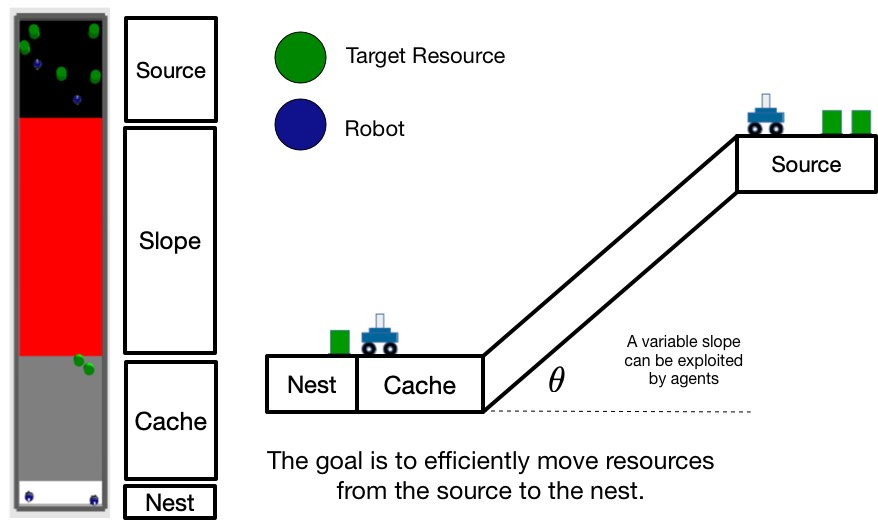
\includegraphics[width=\textwidth]{arena.jpg}
	\caption{Arena Layout}
	\label{fig:arena}
\end{figure}

\begin{figure}
	\centering
	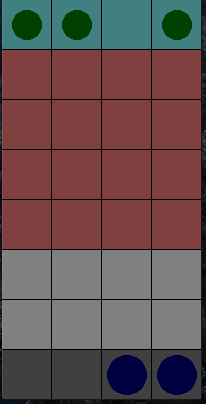
\includegraphics[width=0.3\textwidth]{arena_layout.png}
	\caption{Arena Screenshot}
	\label{fig:arena_2}
\end{figure}

\subsection{Observations and Actions}\label{observation_space}

Agents have a sensing range that indicates how many tiles around them they can observe. 
A sensing range of 0 means an agent can just observe the current tile it is on. 
A range of 1 means it can observe a square centred  on its location that extends 1 tile in each direction (9 tiles total including current tile). 
A range of 2 means it can observe a square extending 2 tiles in each direction (25 tiles total). 
And so on.
We assume our agent represents a robot with only local sensing capabilities and use a sensing range of 1, which has the added benefit of reducing computation.
For each tile in its sensing range, an agent observes a onehotencoded 4-bit vector. 
The values it reads denote the following: Blank= 1000, Agent = 0100, Resource = 0010, Wall = 0001.
Tiles are read row by row from top left to bottom right. 
The next part of an agent's observation is a 4-bit vector denoting which part of the arena it is on, similar to a real robot with a ground sensor that can detect the unique colour of each area.
The values of this vector can be as follows: Nest = 1000, Cache = 0100, Slope = 0010, Source = 0001
The final part of an agent's observation is 1-bit for resource possession. 
The values can be as follows: Has resource = 1, Doesn’t have resource = 0
The total length of the observation vector is 9x4 + 4 + 1= 41 bits.\\

An agent can perform 6 possible actions, represented by the following values: Forward = 0, Backward = 1, Left = 2, Right = 3, Pick-up = 4, Drop = 5.
We use a recurrent neural network to choose actions based on the observed state.
Since many of the positions in the environment will produce the same observation, a recurrent neural network gives the agent a simple form of memory, preventing it from getting "stuck" in infinite state transition loops.
The default network has 41 inputs, 1 bias input and 6 recurrent inputs (one for each of the 6 outputs). 
There is no hidden layer, just a 6-neuron output layer. 
This makes for a total of (41+1+6)x6 = 288 weights. 
The output layer uses a linear activation function.

\subsection{Team Type and Reward Level}\label{rewards}

During the evolutionary process, it is possible to have four different combinations of team type and reward level that impact evolution.
A team can be either homogeneous, with all agents having the same genome, or it can be heterogeneous, with agents having different genomes.
In our case, a heterogeneous team has two different genomes, with half the team having one genome and the other half of the team having the other.
During evolution, agents can be rewarded as a team or individually, meaning the resource retrieved by an agent can, respectively, count towards the fitness of its teammates or only its own fitness.
In the latter case, an individual agent with a high reward and low cost can be selected while its team-mates are discarded. 
The four combinations are thus: heterogeneous team with team rewards (Het-Team), homogeneous team with team rewards (Hom-Team), heterogeneous team with individual rewards (Het-Ind) and homogeneous team with individual rewards (Hom-Ind).\\

For the purposes of this analysis, we only use the Het-Team configuration.

\section{Additional Experiments}

In the following, we show experimental results that were not included in the main report.

\subsection{FFNN}\label{FFNN}

The scores for FFNNs all fall into the leftmost bucket of the distribution plot as we see in Figure \ref{fig:ffnn_linear}. We also see that the mean curve is very flat, with very little variance. FFNN solutions are consistently poor, indicating, as mentioned in the main text of the report, that RNNs might be necessary to solve the problem.

\begin{figure}[!tbp]
  \centering
  % FFNN no-bias 0HL
%  \subfloat{\includegraphics[width=0.3\textwidth]{ffnn_no-bias_0HL/ffnn_no-%bias_0HL_score_trials_ordered_.png}}
%  \hfill
%  \subfloat{\includegraphics[width=0.3\textwidth]{ffnn_no-bias_0HL/ffnn_no-%bias_0HL_variance_meanscore_.png}}
%  \hfill
%  \subfloat{\includegraphics[width=0.3\textwidth]{ffnn_no-bias_0HL/ffnn_no-%bias_0HL_all_scores_log_dist_.png}}
  
% FFNN bias 0HL
  \subfloat{\includegraphics[width=0.3\textwidth]{ffnn_bias_0HL/ffnn_bias_0HL_score_trials_ordered_.png}}
  \hfill
  \subfloat{\includegraphics[width=0.3\textwidth]{ffnn_bias_0HL/ffnn_bias_0HL_variance_meanscore_.png}}
  \hfill
  \subfloat{\includegraphics[width=0.3\textwidth]{ffnn_bias_0HL/ffnn_bias_0HL_all_scores_log_dist_.png}}
  
  \caption{FFNN with linear activation}
  \label{fig:ffnn_linear}
\end{figure}

%%%



\section{FFNN w/ Non-linear Activation} \label{ffnn_non-linear}
\begin{figure}[!tbp]
  \centering
  % FFNN no-bias 0HL
  \subfloat{\includegraphics[width=0.3\textwidth]{ffnn_no-bias_0HL_tanh/ffnn_no-bias_0HL_tanh_score_trials_ordered_.png}}
  \hfill
  \subfloat{\includegraphics[width=0.3\textwidth]{ffnn_no-bias_0HL_tanh/ffnn_no-bias_0HL_tanh_variance_meanscore_.png}}
  \hfill
  \subfloat{\includegraphics[width=0.3\textwidth]{ffnn_no-bias_0HL_tanh/ffnn_no-bias_0HL_tanh_all_scores_log_dist_.png}}
  
  % FFNN no-bias 1HL
  \subfloat{\includegraphics[width=0.3\textwidth]{ffnn_no-bias_1HL_4HU_tanh/ffnn_no-bias_1HL_4HU_tanh_score_trials_ordered_.png}}
  \hfill
  \subfloat{\includegraphics[width=0.3\textwidth]{ffnn_no-bias_1HL_4HU_tanh/ffnn_no-bias_1HL_4HU_tanh_variance_meanscore_.png}}
  \hfill
  \subfloat{\includegraphics[width=0.3\textwidth]{ffnn_no-bias_1HL_4HU_tanh/ffnn_no-bias_1HL_4HU_tanh_all_scores_log_dist_.png}}

% FFNN no-bias 2HL
  \subfloat{\includegraphics[width=0.3\textwidth]{ffnn_no-bias_2HL_4HU_tanh/ffnn_no-bias_2HL_4HU_tanh_score_trials_ordered_.png}}
  \hfill
  \subfloat{\includegraphics[width=0.3\textwidth]{ffnn_no-bias_2HL_4HU_tanh/ffnn_no-bias_2HL_4HU_tanh_variance_meanscore_.png}}
  \hfill
  \subfloat{\includegraphics[width=0.3\textwidth]{ffnn_no-bias_2HL_4HU_tanh/ffnn_no-bias_2HL_4HU_tanh_all_scores_log_dist_.png}}
  
% FFNN bias 0HL
  \subfloat{\includegraphics[width=0.3\textwidth]{ffnn_bias_0HL_tanh/ffnn_bias_0HL_tanh_score_trials_ordered_.png}}
  \hfill
  \subfloat{\includegraphics[width=0.3\textwidth]{ffnn_bias_0HL_tanh/ffnn_bias_0HL_tanh_variance_meanscore_.png}}
  \hfill
  \subfloat{\includegraphics[width=0.3\textwidth]{ffnn_bias_0HL_tanh/ffnn_bias_0HL_tanh_all_scores_log_dist_.png}}
  
  % FFNN bias 1HL
  \subfloat{\includegraphics[width=0.3\textwidth]{ffnn_bias_1HL_4HU_tanh/ffnn_bias_1HL_4HU_tanh_score_trials_ordered_.png}}
  \hfill
  \subfloat{\includegraphics[width=0.3\textwidth]{ffnn_bias_1HL_4HU_tanh/ffnn_bias_1HL_4HU_tanh_variance_meanscore_.png}}
  \hfill
  \subfloat{\includegraphics[width=0.3\textwidth]{ffnn_bias_1HL_4HU_tanh/ffnn_bias_1HL_4HU_tanh_all_scores_log_dist_.png}}

% FFNN bias 2HL
  \subfloat{\includegraphics[width=0.3\textwidth]{ffnn_bias_2HL_4HU_tanh/ffnn_bias_2HL_4HU_tanh_score_trials_ordered_.png}}
  \hfill
  \subfloat{\includegraphics[width=0.3\textwidth]{ffnn_bias_2HL_4HU_tanh/ffnn_bias_2HL_4HU_tanh_variance_meanscore_.png}}
  \hfill
  \subfloat{\includegraphics[width=0.3\textwidth]{ffnn_bias_2HL_4HU_tanh/ffnn_bias_2HL_4HU_tanh_all_scores_log_dist_.png}}  
  
  \caption{FFNN with tanh activation}
  \label{fig:ffnn_tanh}	
\end{figure}

\section{RNN with Non-linear Activation and Bias} \label{rnn_non-linear_bias}

\begin{figure}[!tbp]
  \centering
  
% RNN bias 0HL
  \subfloat{\includegraphics[width=0.3\textwidth]{rnn_bias_0HL_tanh/rnn_bias_0HL_tanh_score_trials_ordered_.png}}
  \hfill
  \subfloat{\includegraphics[width=0.3\textwidth]{rnn_bias_0HL_tanh/rnn_bias_0HL_tanh_variance_meanscore_.png}}
  \hfill
  \subfloat{\includegraphics[width=0.3\textwidth]{rnn_bias_0HL_tanh/rnn_bias_0HL_tanh_all_scores_log_dist_.png}}
  
  % RNN bias 1HL
  \subfloat{\includegraphics[width=0.3\textwidth]{rnn_bias_1HL_4HU_tanh/rnn_bias_1HL_4HU_tanh_score_trials_ordered_.png}}
  \hfill
  \subfloat{\includegraphics[width=0.3\textwidth]{rnn_bias_1HL_4HU_tanh/rnn_bias_1HL_4HU_tanh_variance_meanscore_.png}}
  \hfill
  \subfloat{\includegraphics[width=0.3\textwidth]{rnn_bias_1HL_4HU_tanh/rnn_bias_1HL_4HU_tanh_all_scores_log_dist_.png}}

% RNN bias 2HL
  \subfloat{\includegraphics[width=0.3\textwidth]{rnn_bias_2HL_4HU_tanh/rnn_bias_2HL_4HU_tanh_score_trials_ordered_.png}}
  \hfill
  \subfloat{\includegraphics[width=0.3\textwidth]{rnn_bias_2HL_4HU_tanh/rnn_bias_2HL_4HU_tanh_variance_meanscore_.png}}
  \hfill
  \subfloat{\includegraphics[width=0.3\textwidth]{rnn_bias_2HL_4HU_tanh/rnn_bias_2HL_4HU_tanh_all_scores_log_dist_.png}}  
  
  \caption{RNN with tanh activation and bias}
  \label{fig:rnn_tanh_bias}	
\end{figure}	

\begin{figure}[!tbp]
  \centering
  
% RNN bias 0HL
  \subfloat{\includegraphics[width=0.3\textwidth]{rnn_bias_0HL_relu/rnn_bias_0HL_relu_score_trials_ordered_.png}}
  \hfill
  \subfloat{\includegraphics[width=0.3\textwidth]{rnn_bias_0HL_relu/rnn_bias_0HL_relu_variance_meanscore_.png}}
  \hfill
  \subfloat{\includegraphics[width=0.3\textwidth]{rnn_bias_0HL_relu/rnn_bias_0HL_relu_all_scores_log_dist_.png}}
  
  % RNN bias 1HL
  \subfloat{\includegraphics[width=0.3\textwidth]{rnn_bias_1HL_4HU_relu/rnn_bias_1HL_4HU_relu_score_trials_ordered_.png}}
  \hfill
  \subfloat{\includegraphics[width=0.3\textwidth]{rnn_bias_1HL_4HU_relu/rnn_bias_1HL_4HU_relu_variance_meanscore_.png}}
  \hfill
  \subfloat{\includegraphics[width=0.3\textwidth]{rnn_bias_1HL_4HU_relu/rnn_bias_1HL_4HU_relu_all_scores_log_dist_.png}}

% RNN bias 2HL
  \subfloat{\includegraphics[width=0.3\textwidth]{rnn_bias_2HL_4HU_relu/rnn_bias_2HL_4HU_relu_score_trials_ordered_.png}}
  \hfill
  \subfloat{\includegraphics[width=0.3\textwidth]{rnn_bias_2HL_4HU_relu/rnn_bias_2HL_4HU_relu_variance_meanscore_.png}}
  \hfill
  \subfloat{\includegraphics[width=0.3\textwidth]{rnn_bias_2HL_4HU_relu/rnn_bias_2HL_4HU_relu_all_scores_log_dist_.png}}  
  
  \caption{RNN with ReLU activation and bias}
  \label{fig:rnn_relu_bias}	
\end{figure}	

\begin{figure}[!tbp]
  \centering
  % RNN bias 0HL
  \subfloat{\includegraphics[width=0.3\textwidth]{rnn_bias_0HL_sigmoid/rnn_bias_0HL_sigmoid_score_trials_ordered_.png}}
  \hfill
  \subfloat{\includegraphics[width=0.3\textwidth]{rnn_bias_0HL_sigmoid/rnn_bias_0HL_sigmoid_variance_meanscore_.png}}
  \hfill
  \subfloat{\includegraphics[width=0.3\textwidth]{rnn_bias_0HL_sigmoid/rnn_bias_0HL_sigmoid_all_scores_log_dist_.png}}
  
  % RNN bias 1HL
  \subfloat{\includegraphics[width=0.3\textwidth]{rnn_bias_1HL_4HU_sigmoid/rnn_bias_1HL_4HU_sigmoid_score_trials_ordered_.png}}
  \hfill
  \subfloat{\includegraphics[width=0.3\textwidth]{rnn_bias_1HL_4HU_sigmoid/rnn_bias_1HL_4HU_sigmoid_variance_meanscore_.png}}
  \hfill
  \subfloat{\includegraphics[width=0.3\textwidth]{rnn_bias_1HL_4HU_sigmoid/rnn_bias_1HL_4HU_sigmoid_all_scores_log_dist_.png}}

% RNN bias 2HL
  \subfloat{\includegraphics[width=0.3\textwidth]{rnn_bias_2HL_4HU_sigmoid/rnn_bias_2HL_4HU_sigmoid_score_trials_ordered_.png}}
  \hfill
  \subfloat{\includegraphics[width=0.3\textwidth]{rnn_bias_2HL_4HU_sigmoid/rnn_bias_2HL_4HU_sigmoid_variance_meanscore_.png}}
  \hfill
  \subfloat{\includegraphics[width=0.3\textwidth]{rnn_bias_2HL_4HU_sigmoid/rnn_bias_2HL_4HU_sigmoid_all_scores_log_dist_.png}}  
  
  \caption{RNN with sigmoid activation and bias}
  \label{fig:rnn_sigmoid_bias}	
\end{figure}	

\end{appendices}
\end{document}
